% Подсекция 3.1.x: Применение INTENSE к нейронам РНС
% Источник: Kononov2025
% Методы GCMI и статтестирования описаны в sec:intense_gcmi и sec:intense_stat — НЕ дублировать.

\subsection{Результаты анализа селективности искусственных нейронов в задаче контекстно-зависимого принятия решений}\label{sec:intense_rnn}

Метод INTENSE, описанный в предыдущих секциях, был применён не только к биологическим нейронам, но и к скрытым единицам рекуррентной нейронной сети (РНС), обученной задаче контекстно-зависимого принятия решений (подробное описание задачи и популяционного анализа приведено в секции~\ref{sec:rnn}). Целью данного анализа являлась верификация функциональных ролей нейронов, классифицированных по популяциям на основе шаблонного метода (уравнение~\eqref{eq:rnn_population}), с помощью независимого информационно-теоретического критерия.

Для каждого из 250 скрытых нейронов РНС была вычислена взаимная информация между его активацией и знаком первичной когерентности стимула с использованием оценщика GCMI (секция~\ref{sec:intense_gcmi}). Статистическая значимость оценивалась посредством пермутационного тестирования (10\,000 суррогатов) с поправкой Холма на множественные сравнения ($\alpha = 0{,}01$), аналогично процедуре, описанной в секции~\ref{sec:intense_stat}.

Результаты подтвердили, что динамически определённые популяции несут различные функциональные роли (рис.~\ref{fig:rnn_mi}): нейроны популяции $\mathrm{G}_+$ кодировали информацию о положительной когерентности стимула, а $\mathrm{G}_-$~--- об отрицательной. Кроме того, анализ выявил, что популяция $\mathrm{G}_a$, первоначально классифицированная как <<активная при любом стимуле>>, содержит непересекающиеся подгруппы нейронов с противоположными стимульными предпочтениями. Этот результат, невидимый при популяционном анализе, указывает на механизм контекстно-зависимой маршрутизации информации внутри данной популяции.

\begin{figure}[ht]
\centering
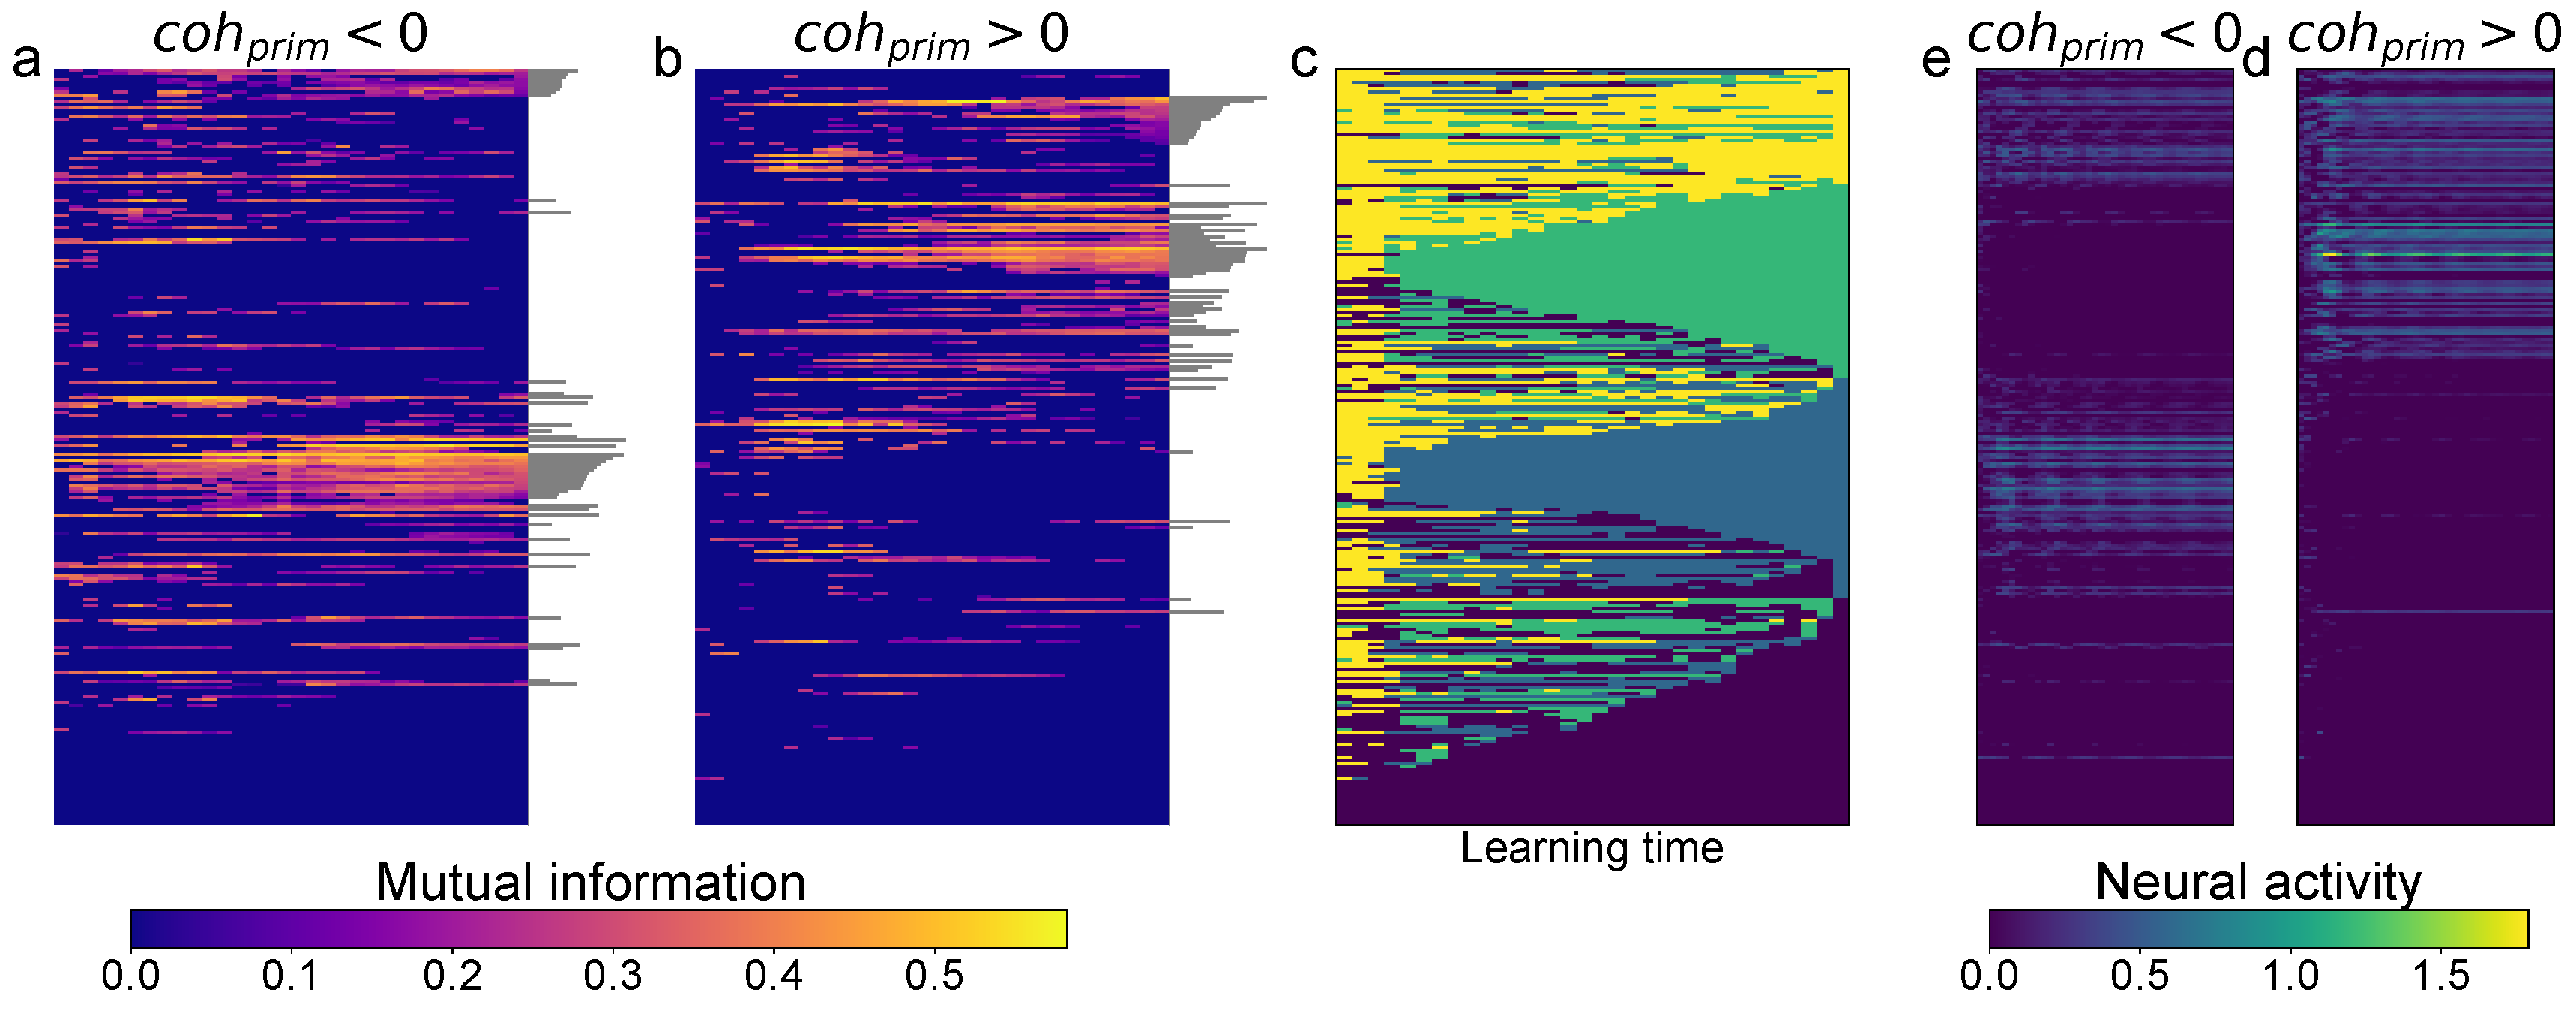
\includegraphics[width=\textwidth]{images/rnn/fig_mi.pdf}
\caption{Верификация функциональных ролей популяций РНС с помощью взаимной информации.
(a,\,b)~ВИ между активностью отдельных нейронов и знаком первичной когерентности для двух моментов пробы. Цветные полосы~--- статистически значимые значения (пермутационный тест, $p < 0{,}01$ с поправкой Холма).
(c)~Принадлежность нейронов к четырём популяциям.
(d,\,e)~Примеры селективных ответов отдельных нейронов (среднее $\pm$ ст. ошибка по пробам).
По~\cite{Kononov2025}.}
\label{fig:rnn_mi}
\end{figure}

Таким образом, применение INTENSE к искусственным нейронам демонстрирует универсальность информационно-теоретического подхода: один и тот же метод, разработанный для анализа кальциевых записей биологических нейронов, позволяет выявить функциональную специализацию элементов искусственной нейронной сети и обнаружить тонкую внутреннюю структуру, не доступную при чисто популяционном анализе.

\subsubsection{Краткие выводы}

Разработан информационно-теоретический фреймворк INTENSE для анализа нейронной селективности, обладающий следующими преимуществами:
\begin{itemize}
    \item универсальность в отношении типов нейронных сигналов и поведенческих переменных;
    \item контроль ложных обнаружений через циклические сдвиги, сохраняющие автокорреляцию;
    \item ускорение пермутационного тестирования методом БПФ ($100$--$2500\times$);
    \item разделение истинной смешанной селективности от артефактов, обусловленных корреляциями поведенческих переменных;
    \item валидация на синтетических данных и сопоставление с классическими методами детекции клеток места;
    \item применимость к искусственным нейронным сетям без модификации метода.
\end{itemize}

При применении к гиппокампальным записям фреймворк выявил разнообразные типы селективных нейронов и показал, что примерно треть наблюдаемой мультиселективности объясняется поведенческой избыточностью, а замена ВИ на линейную корреляцию приводит к потере более двух третей значимых ассоциаций. Применение того же метода к искусственной РНС подтвердило функциональные роли динамически определённых популяций и выявило тонкую внутреннюю структуру, недоступную при популяционном анализе.
